\section{Signal Modeling}\label{sec:hmmSig}

This section describes the signal contribution to the various categories defined in Section \ref{sec:hmmBdt}.
The expected signal contribution in each category is modeled in the \muu distribution with the simulated datasets described in Section \ref{sec:hmmSim}.
As the production mechanism is essentially indistinguishable in terms of signal shape, no further effort is made to separate events originating from VH mechanisms from ggF, VBF, or ttH mechanisms.
From this point, the ensemble of production mechanisms is combined and referred to as \emph{signal}.

An empirical functional form is used to parameterize the shape of the signal distribution.
The natural width of the Higgs decay ($\Gamma_\text{H}\approx4$~MeV) is too small to resolve at ATLAS.
The signal shape is consequently determined by the momentum resolution for muons.
As such, a reasonable choice of function is the double sided Crystal Ball (CB) given in Equation \ref{eq:hmmSignal}.
\begin{equation}\label{eq:hmmSignal}
  f_\text{S}(m_{\mu\mu}) =
  \begin{cases}
  \text{CB}_\text{high}(\alpha_\text{high},n_\text{high},\sigma,\bar{x}) & \text{for }m_{\mu\mu}>\bar{x}\\
  \text{CB}_\text{low}(\alpha_\text{low},n_\text{low},\sigma,\bar{x}) & \text{for }m_{\mu\mu}<=\bar{x}\\
  \end{cases}
\end{equation}
Here, $\alpha_\text{low}$ and $\alpha_\text{high}$ values are the cross-over value for the high and low CB functions.
The other parameters are the shared mean and width of the CB functions, $\bar{x}$ and $\sigma$,
while $n_\text{low}$ and $n_\text{high}$ are the powers for the power-law tails of the high and low CB functions.
The CB function itself is defined in Equation \ref{eqn:hmmCb}.
\begin{equation}\label{eqn:hmmCb}
    \text{CB}(x,\alpha,n,\bar{x},\sigma) = 
    \begin{cases}
        \exp{-\frac{(x-\bar{x})^2}{2\sigma^2}} & \text{for }\frac{(x-\bar{x})}{2\sigma}>-\alpha \\
        \left(\frac{n}{|\alpha|}\right)^n \exp{-\frac{|\alpha|}{2}} \left(\frac{n}{|\alpha|}-|\alpha|\right)^{-n} & \text{otherwise}\\
    \end{cases}
\end{equation}
The CB function is normalized when treated as a PDF.
In the signal model, the normalization is scaled to match the expected number of signal events.

The following diagrams in Figure \ref{fig:hmmSignalFit} show fits of the signal model to the simulated distribution, both before and after categorization with the BDT score.
The corresponding fitted values of signal model parameters parameters are listed in Table \ref{tab:hmmSignalFit}.



\afterpage{
\begin{minipage}{\textwidth}
\begin{figure}[H]
  \centering
  \subfloat[][]{{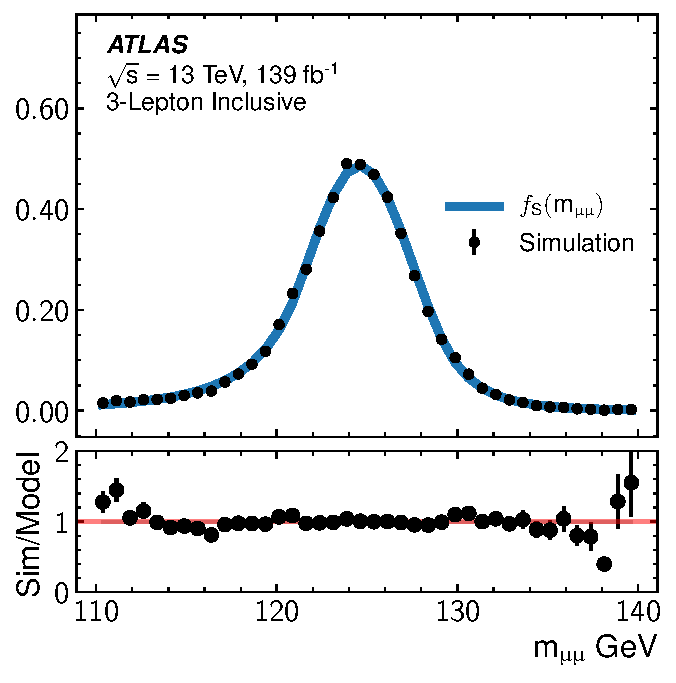
\includegraphics[width=0.30\textwidth]{figures/hmm/signalFits2/sigfit-3lep.pdf}}}
  \subfloat[][]{{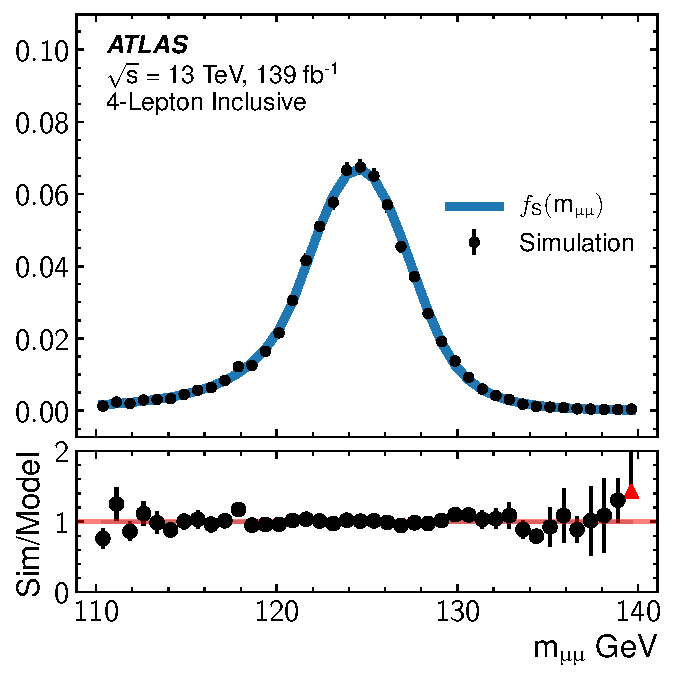
\includegraphics[width=0.30\textwidth]{figures/hmm/signalFits2/sigfit-4lep.pdf}}}\\
  \subfloat[][]{{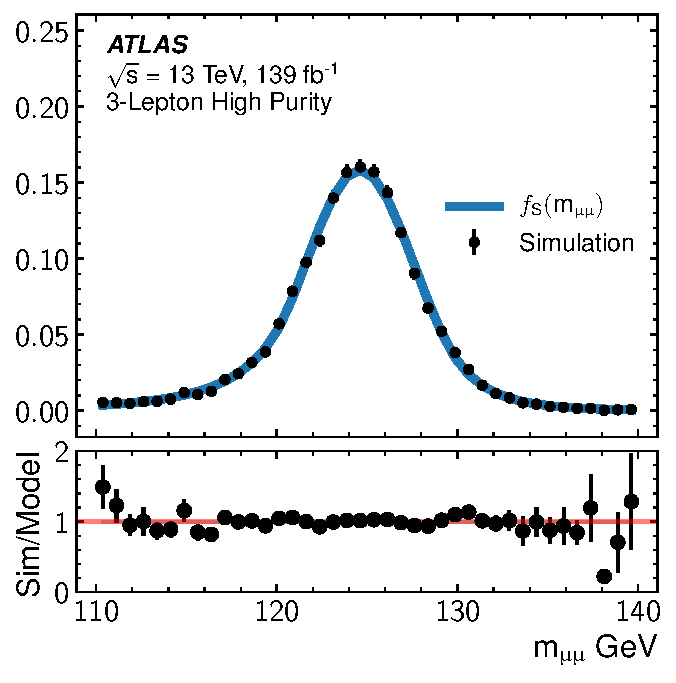
\includegraphics[width=0.30\textwidth]{figures/hmm/signalFits2/sigfit-3lep0.pdf}}}
  \subfloat[][]{{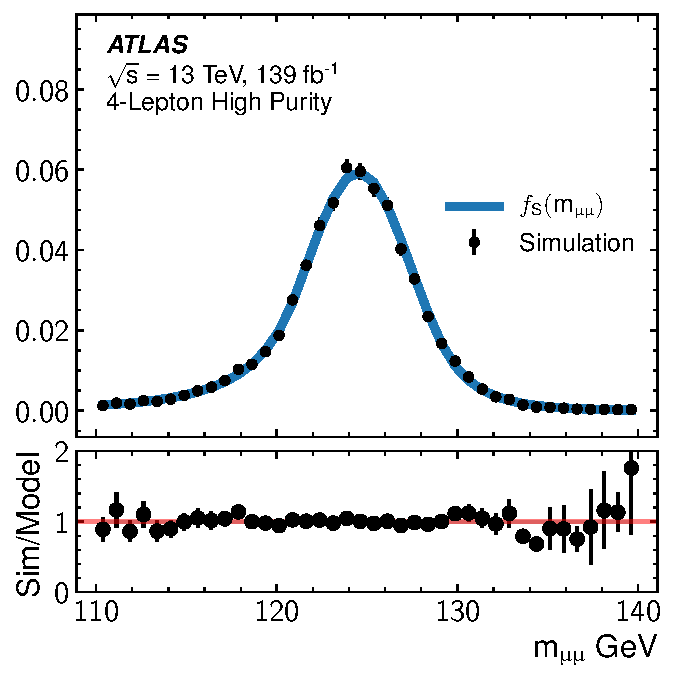
\includegraphics[width=0.30\textwidth]{figures/hmm/signalFits2/sigfit-4lep0.pdf}}}
  \subfloat[][]{{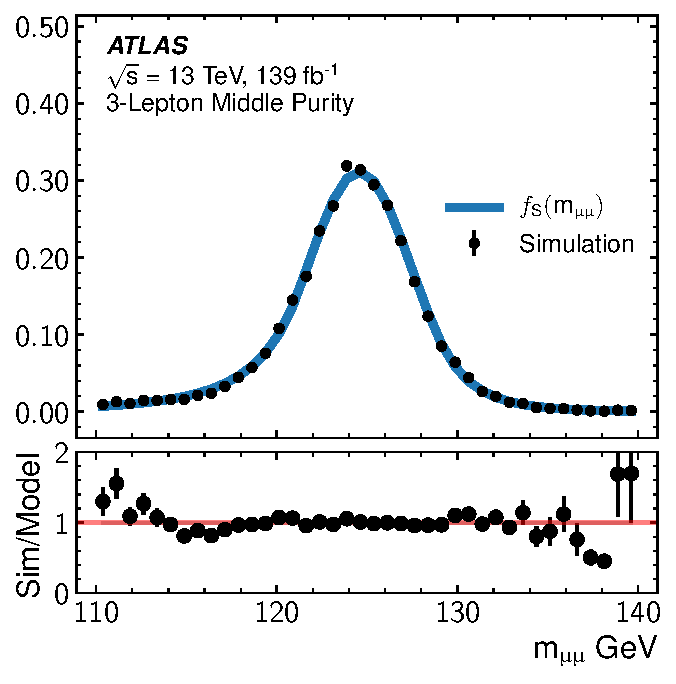
\includegraphics[width=0.30\textwidth]{figures/hmm/signalFits2/sigfit-3lep1.pdf}}}
  \caption{Fits of the signal model to the simulated signal in each categories. 
On top, (a) shows 3-lepton and (b) shows 4-lepton inclusive categories.
Below, (c and d) show 3-lepton HP and MP, and (e) shows 4-lepton LP.
The blue line shows the fitted signal function, while the black dots show the simulation with statistical errors.
}
    \label{fig:hmmSignalFit}
\end{figure}
% #
% \vspace{-2em}
\begin{table}[H]
 \caption{Parameters of the signal model fit to simulation.}
 \begin{center}
\begin{tabular}{l r r r r r}\toprule
Parameter & 4-lepton & 3-lepton & 4-lepton HP & 3-lepton LP & 3-lepton HP \\
\midrule
$\alpha_\text{low}$ & 1.11 & 1.32 & 1.15 & 1.36 & 1.33 \\
$n_\text{high}$ & 15.65 & 26.93 & 13.68 & 23.92 & 58.46 \\
$\bar{x}$ & 124.5 & 124.5 & 124.4 & 124.5 & 124.5 \\
$\alpha_\text{high}$ & 1.43 & 1.48 & 1.51 & 1.50 & 1.41 \\
$\sigma$ & 2.79 & 2.91 & 2.84 & 2.88 & 2.92 \\
$n_\text{low}$ & 4.59 & 2.67 & 4.94 & 2.04 & 2.94 \\
\bottomrule\end{tabular}
 \end{center}
\label{tab:hmmSignalFit}
\end{table}
\end{minipage}
\clearpage
}


\subsection{Signal+Background Model}

It is helpful to define the predictions of various ``signal+background'' (S+B) hypotheses.
This combines the signal prediction from Equation \ref{eq:hmmSignal} with the background prediction in Equation \ref{eqn:hmmBkgFunc}.
The Standard Model predicts a particular signal multiplicity, $N_{SM}$.
The relative amplitude of the signal compared to the prediction of the Standard Model is defined as the \emph{signal strength}, \mus.
A range of S+B hypotheses are possible, labeled by the signal strength.
For example, \mus=1 describes a hypothesis with the Standard Model signal strength, while \mus=0 describes a ``background-only'' (B) hypothesis.

The S+B hypothesis predicts the relative frequency of events as a function of \muu.
It is defined in Equation \ref{eqn:hmmSbFunc} as the sum of the normalized signal shape PDF $f_\text{S}(\muu)$, and the normalized background PDF $f_\text{B}(\muu)$.
\begin{equation}\begin{split}\label{eqn:hmmSbFunc}
f_\text{S+B}(\muu) = N_\text{S}\times f_\text{S}(\muu) + N_\text{B}\times f_\text{B}(\muu)
\end{split}\end{equation} 
There are three free parameters in Equation \ref{eqn:hmmSbFunc}: the shape parameters $a$ and $b$ that describe the background, and $N_\text{S}\equiv\mus\times N_{SM}$ where \mus is free.
Each of these may be adjusted by \code{minuit} to fit the data distribution in each category.
The overall normalization of the function, when treated as a PDF, is normalized as was the case with the background-only function.

In the case that a strong signal is not observed in the data, it is still possible to consider which S+B hypotheses are compatible and incompatible with the observation.
In this case, some set of hypotheses are considered excluded to a particular confidence level.
To this end, an S+B hypothesis is defined by a fixed \mus, and free parameters $a$ and $b$.
